\chapter{Multiplizität, Entropie und Gleichgewicht unter Nebenbedingungen}

\lectureoverview{Eine Wahrscheinlichkeitsverteilung wird zu einem thermodynamischen Objekt, sobald ihre Zustände Energien tragen. Zunächst verknüpfen wir die Zunahme der Entropie mit der Einstellung des Gleichgewichts und verwenden \(dE=T\,dS\), um die Richtung des Wärmeflusses herzuleiten. Anschließend ersetzen wir ein System durch eine große Menge von Replikaten, zählen die Anordnungen, die zu jeder Belegungszahlenverteilung gehören, und zeigen, dass der Logarithmus dieser Multiplizität das \(N\)-Fache der Entropie ist. Das Gleichgewicht ist daher ein Problem der Entropiemaximierung unter Nebenbedingungen. Die dafür erforderliche Methode liefern die Lagrange-Multiplikatoren.}

\section{Die drei grundlegenden Größen}

Sei \(i\) eine Bezeichnung für die diskreten Zustände, die einem System zur Verfügung stehen. Für den Moment ist die Diskretheit hilfreich, weil wir so Zustände zählen können, ohne Phasenraumintegrationsmaße einzuführen. Ist die Wahrscheinlichkeit des Zustands \(i\) gleich \(P_i\), so gilt
\begin{equation}
 \sum_i P_i=1.
 \label{eq:sm3-normalization}
\end{equation}
Ist die Energie dieses Zustands \(E_i\), so beträgt die mittlere Energie
\begin{equation}
 \overline E=\sum_iP_iE_i.
 \label{eq:sm3-mean-energy}
\end{equation}
Das Wort \emph{mittel} ist wichtig. Das System muss den Wert \(\overline E\) nicht in einem einzelnen mikroskopischen Zustand annehmen; es handelt sich um den mit den Wahrscheinlichkeiten gewichteten Mittelwert über die möglichen Werte.

\begin{classroomqa}
\classquestion{Gibt es hier einen sinnvollen Unterschied zwischen Wahrscheinlichkeit und Statistik?}
\lecturerresponse{Die Wahrscheinlichkeit liefert ein Modell möglicher Ergebnisse, während die Statistik gewöhnlich von beobachteten Daten ausgeht und fragt, welche Schlüsse sich daraus ziehen lassen. In der vorliegenden Rechnung verwenden wir Wahrscheinlichkeitsverteilungen, auch wenn dieselben Mittelwerte ganz natürlich in statistischen Daten auftreten. Im informellen Wortwechsel in der Vorlesung werden die Begriffe locker verwendet, weil dieser Unterschied für die folgende Physik keine Rolle spielt.
\lecturetimestamp{00:01:39--00:02:21}}
\end{classroomqa}

Die Entropie der Verteilung ist
\begin{equation}
 S[P]=-\sum_iP_i\log P_i.
 \label{eq:sm3-entropy}
\end{equation}
Dieser Ausdruck ist nichtnegativ. Für jede von null verschiedene Wahrscheinlichkeit gilt
\(0<P_i\leq1\), also \(\log P_i\leq0\); für \(P_i\to0\) gilt der übliche Grenzwert \(P_i\log P_i\to0\).

\begin{figure}[t]
\centering
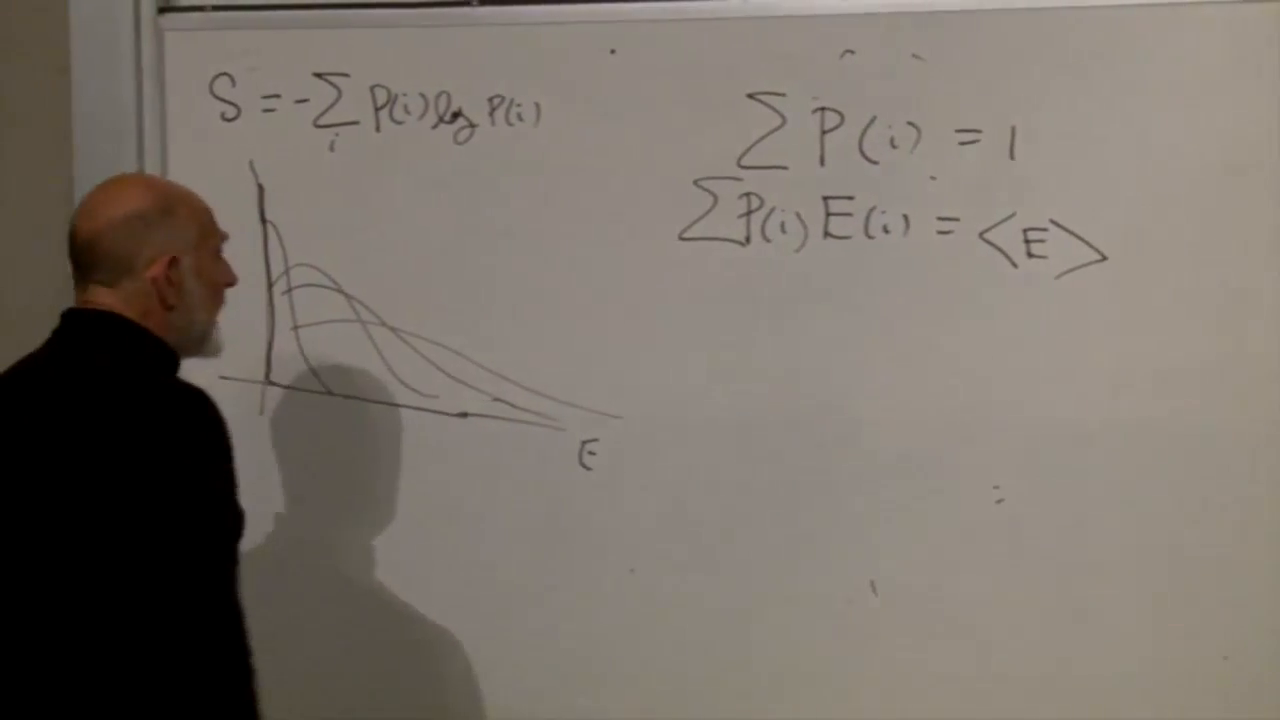
\includegraphics[width=0.88\textwidth]{lecture_03_figure_02.png}
\caption{Die erste Tafelansicht zeigt die Formeln für Entropie, Normierung und mittlere Energie sowie eine qualitative Familie von Gleichgewichtsverteilungen.}
\lectureframe{00:06:44}
\end{figure}

\section{Gleichgewicht als Familie von Verteilungen}

Aus der vorherigen Vorlesung ist eine von einem Parameter abhängige Familie von Gleichgewichtsverteilungen hervorgegangen. Man kann diese Familie durch die Temperatur parametrisieren, doch vorerst ist es nützlicher, sie durch die mittlere Energie \(\overline E\) zu kennzeichnen. Bei der kleinstmöglichen Energie ist die Verteilung auf einen Grundzustand konzentriert:
\[
 P_i=\delta_{i0}.
\]
Dann besteht keine Ungewissheit über den Zustand, und es gilt \(S=0\). Wenn sich die Gleichgewichtsverteilung über mehr Energieniveaus ausbreitet, steigen sowohl ihre mittlere Energie als auch ihre Entropie.

Diese Aussage gilt für die thermische Familie, nicht für jede denkbare Verteilungsfamilie. Eine beliebige Familie könnte sich zu höheren Energien verschieben und zugleich schmaler werden. Die herzuleitenden Gleichgewichtsverteilungen verhalten sich im gewöhnlichen Bereich positiver Temperaturen nicht so. Entlang dieser Familie gilt
\begin{equation}
 \frac{dS}{d\overline E}>0.
 \label{eq:sm3-positive-temperature-branch}
\end{equation}
Systeme mit beschränktem Spektrum können auch Zweige besitzen, auf denen diese Ableitung negativ ist. Diese Bereiche negativer Temperatur sind real, werden im vorliegenden Argument aber zunächst ausgeklammert.

Thermisches Gleichgewicht bedeutet mehr als mikroskopische Ruhe. Moleküle bewegen sich weiter, stoßen zusammen und tauschen Energie aus. Stationär geworden ist die makroskopische Beschreibung: Die Verteilung zeigt keine gerichtete Nettoverschiebung mehr, und getrennte Teile des Systems weisen keinen Nettoenergiefluss mehr auf.

\section{Die thermodynamischen Gesetze in statistischer Sprache}

Der erste Hauptsatz ist die Energieerhaltung. Der zweite Hauptsatz besagt, dass die thermodynamische Entropie eines isolierten makroskopischen Systems nicht abnimmt:
\begin{equation}
 \Delta S_{\mathrm{tot}}\geq0.
 \label{eq:sm3-second-law}
\end{equation}
Gleichheit beschreibt Gleichgewicht oder eine ideal reversible Änderung; bei einer spontanen Relaxation nimmt die Entropie gewöhnlich strikt zu.

In der probabilistischen Beschreibung verteilt sich das Gewicht bei der Relaxation tendenziell auf die makroskopischen Alternativen, die wir weiterhin unterscheiden. Hier ist die in der Vorlesung hervorgehobene Einschränkung wichtig: Wir führen eine \emph{Grobkörnung} durch. Die exakte Hamiltonsche Entwicklung erhält die feinkörnige Phasenraumentropie. Die makroskopische Entropie wächst, weil wir mikroskopische Korrelationen und Einzelheiten nicht mehr verfolgen. Dieser Informationsverlust verbreitert die reduzierte Beschreibung. Eine spontane Verengung würde hingegen bedeuten, dass wir ohne Messung mikroskopische Information erlangt hätten.

Das nullte Gesetz besagt, dass Systeme thermisches Gleichgewicht erreichen können und dass die Gleichgewichtsrelation transitiv ist. Befindet sich \(A\) mit \(B\) im Gleichgewicht und \(B\) mit \(C\), so befindet sich \(A\) mit \(C\) im Gleichgewicht. Die Temperatur liefert die Größe, die diese Transitivität unmittelbar sichtbar macht:
\[
 T_A=T_B,\qquad T_B=T_C
 \quad\Longrightarrow\quad
 T_A=T_C.
\]
Außerhalb des Gleichgewichts fließt Energie vom Teilsystem mit der höheren Temperatur zum Teilsystem mit der niedrigeren Temperatur. Bei gleichen Temperaturen kommt der Nettofluss zum Erliegen. Nun leiten wir diese operationale Aussage aus der Entropiedefinition der Temperatur her.

\section{Warum Energie von warm nach kalt fließt}

Betrachten wir zwei schwach gekoppelte Teilsysteme \(A\) und \(B\). Jedes befindet sich intern im Gleichgewicht, aber ihre Temperaturen unterscheiden sich. Die Bezeichnungen seien so gewählt, dass
\begin{equation}
 T_B>T_A>0.
 \label{eq:sm3-temperature-order}
\end{equation}
Bei einem kleinen Energieaustausch folgt aus der Energieerhaltung für das Gesamtsystem
\begin{equation}
 dE_A+dE_B=0.
 \label{eq:sm3-energy-conservation}
\end{equation}
Der zweite Hauptsatz verlangt
\begin{equation}
 dS_A+dS_B\geq0.
 \label{eq:sm3-entropy-change}
\end{equation}
Für jedes Teilsystem, das intern im Gleichgewicht ist, ist die Temperatur definiert durch
\begin{equation}
 dE_X=T_X\,dS_X,
 \qquad X=A,B.
 \label{eq:sm3-temperature-differential}
\end{equation}
Einsetzen in \eqref{eq:sm3-energy-conservation} ergibt
\begin{equation}
 T_A\,dS_A+T_B\,dS_B=0,
\end{equation}
und damit
\begin{equation}
 dS_B=-\frac{T_A}{T_B}\,dS_A.
 \label{eq:sm3-dsb}
\end{equation}
Setzen wir dieses Ergebnis in \eqref{eq:sm3-entropy-change} ein, so erhalten wir
\begin{align}
 dS_{\mathrm{tot}}
 &=dS_A-\frac{T_A}{T_B}dS_A\\
 &=\frac{T_B-T_A}{T_B}\,dS_A\geq0.
 \label{eq:sm3-flow-entropy}
\end{align}
Da \(T_B-T_A>0\) und \(T_B>0\) gilt, muss für einen spontanen Austausch
\[
 dS_A>0.
\]
Aus Gleichung \eqref{eq:sm3-temperature-differential} folgt dann
\begin{equation}
 dE_A=T_A\,dS_A>0,
 \qquad
 dE_B=-dE_A<0.
 \label{eq:sm3-hot-to-cold}
\end{equation}
Energie ist von \(B\), dem heißeren Teilsystem, zu \(A\), dem kälteren Teilsystem, geflossen. Wärme ist hier einfach Energie im Transit. Der Fluss hält an, bis \(T_A=T_B\) gilt; dann begünstigt die Entropieänderung erster Ordnung keine der beiden Richtungen mehr.

Dasselbe Ergebnis lässt sich in einer Zeile darstellen:
\begin{equation}
 dS_{\mathrm{tot}}
 =dE_A\left(\frac{1}{T_A}-\frac{1}{T_B}\right)\geq0.
 \label{eq:sm3-compact-flow}
\end{equation}
Das Vorzeichen der Differenz der inversen Temperaturen legt das Vorzeichen von \(dE_A\) fest. Diese kompakte Form wird sich später natürlich in das kanonische Ensemble einfügen.

\begin{classroomqa}
\audiencequestion{Setzt dieses Argument voraus, dass \(A\) und \(B\) jeweils bereits im inneren Gleichgewicht sind?}
\lecturerresponse{Ja. Die Zuweisung einer einzelnen Temperatur \(T_A\) beziehungsweise \(T_B\) setzt das voraus. Ist ein Teilsystem intern nicht im Gleichgewicht, teilt man es in kleinere Bereiche auf und wendet das Argument dort lokal an, wo sich eine Temperatur definieren lässt. Die globale Relaxation setzt sich dann aus Energieaustausch zwischen diesen Bereichen zusammen.
\lecturetimestamp{00:24:38--00:25:22}}
\end{classroomqa}

\section{Was gilt als Zustand?}

Bevor wir nach den Gleichgewichtswahrscheinlichkeiten fragen, müssen wir wissen, was die Bezeichnung \(i\) bedeutet. Ein mikroskopischer Zustand ist die vollständigste Beschreibung des Systems, die nach den zugrunde liegenden physikalischen Gesetzen möglich ist. In der klassischen Mechanik stellt man sich die Orte und Impulse aller Teilchen vor. In der Quantenmechanik ist ein Zustand stattdessen ein vollständiger Quantenzustand; die Unschärferelation verhindert eine gleichzeitige scharfe Festlegung sämtlicher klassischer Orte und Impulse.

Für ein Quantensystem in einer endlichen Box kann die relevante Zustandszählung diskret sein. Die klassische statistische Mechanik ergibt sich in einem geeigneten Grenzfall, in dem Summen über dicht liegende Quantenzustände in Phasenraumintegrale übergehen. Dieser Grenzübergang führt auch die Phasenraumzelle ein, die benötigt wird, um die kontinuierliche Entropie dimensionslos zu machen; sie ergibt sich nicht einfach dadurch, dass man ein Summenzeichen durch ein Integralzeichen ersetzt.

\begin{classroomqa}
\audiencequestion{Sollte man sich bei einem Gas einen Zustand als Ort und Impuls jedes einzelnen Moleküls vorstellen?}
\lecturerresponse{Das ist das richtige klassische Bild. Allgemeiner bezeichnet ein Zustand alles, was nach den physikalischen Gesetzen prinzipiell über das System bekannt sein kann. Die Quantenmechanik verändert die Form dieser maximalen Beschreibung und führt zu einer diskreten Zählung bei endlichem Volumen. Das klassische Integral aus der Quantensumme zurückzugewinnen, ist ein echter Grenzübergang und keine Substitution in einer Zeile.
\lecturetimestamp{00:25:31--00:27:38}}
\end{classroomqa}

\section{Ein Wärmebad aus Replikaten}

Die schwierige Frage lässt sich nun nicht mehr umgehen: Was bestimmt \(P_i\), nachdem sich das Gleichgewicht eingestellt hat?

Bringen wir das Teilsystem mit einem sehr großen Wärmebad in Kontakt. Energie kann hin und her fließen, doch das Bad hat so viele Freiheitsgrade, dass die Übertragung einer kleinen Energiemenge seine Temperatur kaum verändert. Ein besonders praktisches Bad besteht aus vielen schwach gekoppelten Replikaten des Teilsystems selbst. Ein Replikat ist das untersuchte System; die übrigen bilden seine Umgebung.

Diese Konstruktion bildet oft ein reales makroskopisches System nach. Man teile einen großen, annähernd homogenen Körper in viele ähnliche Zellen. Jede Zelle ist ein Teilsystem, und die übrigen Zellen bilden ihr Bad. Die Gesamtzahl der Replikate sei \(N\). Die Vorlesungsdemonstration verwendet neun Replikate und drei farblich gekennzeichnete Zustände; die Zählung hängt jedoch nicht von diesen konkreten Zahlen ab.

Sei \(n_i\) die Anzahl der Replikate im Zustand \(i\). Diese Größen heißen \emph{Belegungszahlen}. Es kann unendlich viele mögliche Energieniveaus geben, aber bei endlicher Gesamtenergie sind die Belegungszahlen der sehr hohen Niveaus meist vernachlässigbar oder gleich null.

Die erste Nebenbedingung betrifft schlicht die Zahl der Replikate:
\begin{equation}
 \sum_i n_i=N.
 \label{eq:sm3-number-constraint}
\end{equation}
Die zweite betrifft die Gesamtenergie:
\begin{equation}
 \sum_i n_iE_i=N\overline E.
 \label{eq:sm3-total-energy-constraint}
\end{equation}
Die rechte Seite ist eine extensive Größe. Verdoppelt man die Zahl der Replikate bei gleichbleibendem statistischem Zustand, so verdoppelt sich die Gesamtenergie, während die mittlere Energie pro Replikat \(\overline E\) bleibt.

\begin{classroomqa}
\audiencequestion{Muss die Replikatkonstruktion auch eine Energiebedingung erfüllen?}
\lecturerresponse{Ja. Die Belegungszahlen müssen sich zu \(N\) summieren, und ihre mit der Energie gewichtete Summe muss gleich der festgelegten Gesamtenergie \(N\overline E\) sein. Genau diese beiden Nebenbedingungen schränken später das Entropiemaximum ein.
\lecturetimestamp{00:37:12--00:39:54}}
\end{classroomqa}

Die Wahrscheinlichkeit, dass ein zufällig ausgewähltes Replikat den Zustand \(i\) einnimmt, ist seine relative Häufigkeit:
\begin{equation}
 P_i=\frac{n_i}{N},
 \qquad
 n_i=NP_i.
 \label{eq:sm3-frequency-probability}
\end{equation}

\begin{figure}[t]
\centering
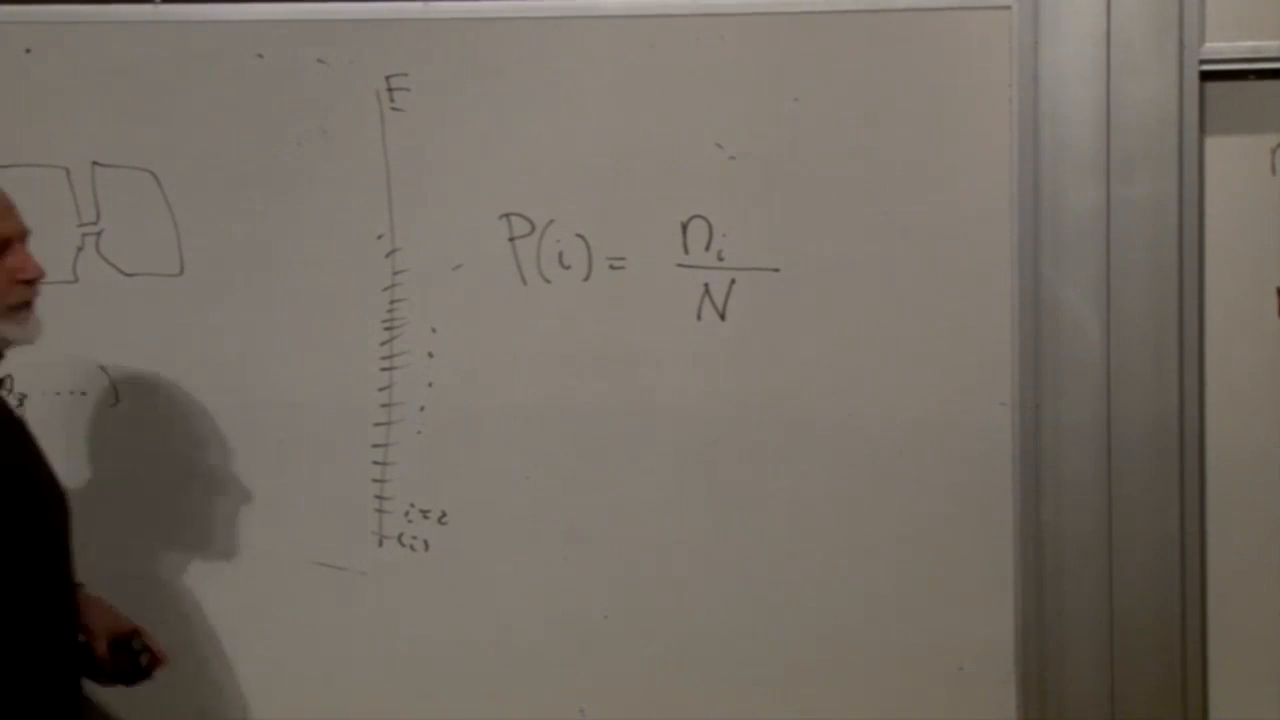
\includegraphics[width=0.82\textwidth]{lecture_03_figure_03.png}
\caption{Das Energieniveaubild und die Identifikation der Wahrscheinlichkeit mit dem Belegungsanteil \(P_i=n_i/N\)}
\lectureframe{00:41:40}
\end{figure}

\begin{classroomqa}
\audiencequestion{Soll die Schreibweise \(N(i)\) an der Tafel etwas anderes bezeichnen als \(n_i\)?}
\lecturerresponse{Nein. Beide bezeichnen die Belegungszahl des Zustands \(i\). Wir verwenden durchgängig \(n_i\) und reservieren das große \(N\) für die Gesamtzahl der Replikate.
\lecturetimestamp{00:41:28--00:41:33}}
\end{classroomqa}

Teilt man \eqref{eq:sm3-number-constraint} und \eqref{eq:sm3-total-energy-constraint} durch \(N\), so erhält man wieder die Wahrscheinlichkeitsbedingungen:
\begin{equation}
 \sum_iP_i=1,
 \qquad
 \sum_iP_iE_i=\overline E.
 \label{eq:sm3-probability-constraints}
\end{equation}
Die Häufigkeitsinterpretation im Ensemble liefert somit wieder die Gleichungen, mit denen wir begonnen haben.

\section{Multiplizität eines Belegungsmusters}

Wir legen einen Satz von Belegungszahlen \(\{n_i\}\) fest. Wie viele Zuordnungen der \(N\) unterscheidbaren Replikate zu den Zuständen ergeben genau diesen Satz? Die Antwort lautet: der Multinomialkoeffizient
\begin{equation}
 C(\{n_i\})=\frac{N!}{\prod_i n_i!}.
 \label{eq:sm3-multiplicity}
\end{equation}
Um den Nenner zu verstehen, ordnen wir zunächst alle \(N\) markierten Replikate auf \(N!\) verschiedene Arten an. Eine Permutation der \(n_i\) Replikate, die denselben Zustand einnehmen, ergibt keine neue Belegungszuordnung. Daher teilen wir für jeden Zustand durch \(n_i!\).

\begin{figure}[t]
\centering
\includegraphics[width=0.88\textwidth]{lecture_03_figure_04.png}
\caption{Die an der Tafel notierte Multinomialmultiplizität \(C=N!/\prod_i n_i!\)}
\lectureframe{00:46:55}
\end{figure}

Unbesetzte Niveaus bereiten kein Problem, denn \(0!=1\). Besetzen alle Replikate einen Zustand, so gilt erwartungsgemäß
\[
 C=\frac{N!}{N!}=1,
\]
Besetzen drei Replikate drei verschiedene, festgelegte Zustände, so gilt
\[
 C=\frac{3!}{1!\,1!\,1!}=6.
\]
Besetzen zwei Replikate zwei festgelegte Zustände, liefert die Formel zwei Zuordnungen: Man vertauscht, welches markierte Replikat welchen Zustand einnimmt.

\begin{classroomqa}
\audiencequestion{Kann mehr als ein Satz von Belegungszahlen die beiden Nebenbedingungen erfüllen?}
\lecturerresponse{In der Regel gibt es viele solche Sätze. Gleichung \eqref{eq:sm3-multiplicity} zählt zunächst die Anordnungen für einen einzelnen festgelegten Satz \(\{n_i\}\), ohne bereits zu entscheiden, ob dieser die Nebenbedingungen erfüllt. Im nächsten Schritt vergleichen wir alle mit den Nebenbedingungen verträglichen Sätze und bestimmen, welcher davon die größte Multiplizität hat.
\lecturetimestamp{00:48:07--00:48:43}}
\end{classroomqa}

Die statistische Annahme lautet, dass die mit dem isolierten Aufbau verträglichen mikroskopischen Zuordnungen gleichberechtigt behandelt werden. Ein makroskopisches Belegungsmuster, das durch mehr Zuordnungen realisiert wird, ist daher wahrscheinlicher. Für großes \(N\) wird die Verteilung der Anteile \(n_i/N\) stark um einen Wert konzentriert. Die Gleichgewichtsanteile sind die Werte, die \(C\) maximieren, unter den Nebenbedingungen \eqref{eq:sm3-number-constraint} und \eqref{eq:sm3-total-energy-constraint}.

\section{Die Stirling-Näherung}

Fakultäten werden schon lange bevor \(N\) makroskopisch groß ist enorm, daher betrachten wir ihre Logarithmen. Wir beginnen mit
\begin{equation}
 \log N!=\sum_{x=1}^{N}\log x.
 \label{eq:sm3-log-factorial-sum}
\end{equation}
Für großes \(N\) wird die Summe durch den Flächeninhalt unter \(\log x\) angenähert:
\begin{align}
 \log N!
 &\simeq\int_1^N\log x\,dx\\
 &=\left[x\log x-x\right]_1^N\\
 &=N\log N-N+1.
 \label{eq:sm3-stirling-integral}
\end{align}
Die Stammfunktion ergibt sich unmittelbar aus
\[
 \frac{d}{dx}(x\log x-x)=\log x.
\]
In führender extensiver Ordnung kann die additive Konstante weggelassen werden:
\begin{equation}
 \log N!\simeq N\log N-N.
 \label{eq:sm3-stirling-log}
\end{equation}
Durch Exponenzieren erhalten wir die in der Vorlesung verwendete vereinfachte Form,
\begin{equation}
 N!\simeq N^N e^{-N}.
 \label{eq:sm3-stirling-simple}
\end{equation}

\begin{figure}[t]
\centering
\includegraphics[width=0.88\textwidth]{lecture_03_figure_05.png}
\caption{Die führende Stirling-Näherung und ihre Herleitung, bei der die Summe von \(\log x\) durch ein Integral ersetzt wird.}
\lectureframe{01:03:45}
\end{figure}

\begin{classroomqa}
\audiencequestion{Bleibt bei der Auswertung von \(x\log x-x\) an der unteren Grenze ein zusätzliches \(+1\) übrig?}
\lecturerresponse{Ja. Gleichung \eqref{eq:sm3-stirling-integral} enthält diese Konstante. Sie ist gegenüber den zu \(N\) proportionalen Termen vernachlässigbar, wenn \(N\to\infty\), weshalb sie in der führenden Näherung weggelassen wird. Die Summe selbst muss bei \(x=1\) beginnen; \(\log0\) ist nicht definiert.
\lecturetimestamp{01:04:12--01:04:35}}
\end{classroomqa}

\begin{classroomqa}
\audiencequestion{Fehlt auch ein Faktor proportional zu \(\sqrt{N}\)?}
\lecturerresponse{Ja. Die genauere asymptotische Formel lautet
\[
 N!\sim\sqrt{2\pi N}\left(\frac{N}{e}\right)^N.
\]
Ihr Logarithmus liefert lediglich den Zusatzterm \(\tfrac12\log(2\pi N)\), der gegenüber \(N\log N-N\) subextensiv ist. Für genaue Wahrscheinlichkeiten bei endlichem \(N\) ist er relevant, nicht aber für die führende Entropieberechnung eines makroskopischen Systems.
\lecturetimestamp{01:04:35--01:05:40}}
\end{classroomqa}

Auch im Nenner von \eqref{eq:sm3-multiplicity} muss die Stirling-Näherung mit Bedacht angewendet werden. Im thermodynamischen Grenzfall gilt für die Zustände mit nichtverschwindenden Grenzwahrscheinlichkeiten \(n_i=NP_i\), sodass ihre Belegungszahlen mit \(N\) anwachsen. Zustände mit sehr kleiner oder verschwindender Belegung lassen sich mithilfe einer Abschneidung bei endlicher Energie behandeln, die man anschließend im Grenzfall wieder aufhebt. Die führende extensive Entropie bleibt von den weggelassenen Termen höherer Ordnung unberührt.

\section{Der Logarithmus der Multiplizität ist die Entropie}

Wenden wir \eqref{eq:sm3-stirling-simple} auf den Zähler und alle makroskopisch besetzten Faktoren im Nenner an:
\begin{equation}
 C\simeq
 \frac{N^Ne^{-N}}
 {\prod_i n_i^{\,n_i}e^{-n_i}}.
 \label{eq:sm3-c-stirling}
\end{equation}
Da \(\sum_i n_i=N\), kürzen sich die führenden Exponentialfaktoren heraus:
\begin{equation}
 C\simeq\frac{N^N}{\prod_i n_i^{\,n_i}}.
 \label{eq:sm3-c-leading}
\end{equation}
Der Logarithmus lässt sich leichter maximieren als ein Produkt; außerdem ist er monoton. Daher treten beide Maxima beim selben Belegungsmuster auf:
\begin{equation}
 \log C=N\log N-\sum_i n_i\log n_i.
 \label{eq:sm3-logc-occupations}
\end{equation}
Setzen wir nun \(n_i=NP_i\) ein:
\begin{align}
 \log C
 &=N\log N-\sum_iNP_i\log(NP_i)\\
 &=N\log N-N\sum_iP_i\log N
   -N\sum_iP_i\log P_i\\
 &=-N\sum_iP_i\log P_i,
 \label{eq:sm3-logc-entropy-derivation}
\end{align}
wobei sich die beiden Terme \(N\log N\) aufgrund der Normierung aufheben. Somit gilt in führender Ordnung für \(N\)
\begin{equation}
 \boxed{\log C=NS}.
 \label{eq:sm3-logc-ns}
\end{equation}

\begin{figure}[t]
\centering
\includegraphics[width=0.88\textwidth]{lecture_03_figure_06.png}
\caption{Die Tafelausführung, die \(\log C=N\log N-\sum_i n_i\log n_i\) mit \(-N\sum_iP_i\log P_i=NS\) verknüpft.}
\lectureframe{01:16:10}
\end{figure}

Diese Beziehung bildet den begrifflichen Kern des Kapitels. Die Entropie ist keine zusätzliche Größe, die dem Zählproblem äußerlich auferlegt wird. Sie ist die logarithmisch gemessene Multiplizität pro Replikat. Die Zahl der mikroskopischen Anordnungen zu maximieren, ist daher in führender Ordnung gleichbedeutend damit, die Entropie eines einzelnen Replikats zu maximieren.

\begin{classroomqa}
\audiencequestion{Wäre die Multiplizität nicht am größten, wenn alle Belegungszahlen gleich wären?}
\lecturerresponse{Bei einer endlichen Zahl von Zuständen ist die Verteilung gleichförmig, wenn kein Zustand ausgezeichnet ist und nur \(\sum_i n_i=N\) vorgegeben wird. Die Bedingung fester Energie ändert das Ergebnis, weil die Werte \(E_i\) verschieden sind. Gleiche Belegungszahlen ergeben im Allgemeinen nicht die vorgegebene mittlere Energie.
\lecturetimestamp{01:17:07--01:18:20}}
\end{classroomqa}

\begin{classroomqa}
\audiencequestion{Das große \(N\) ist zwar groß, aber warum darf die Stirling-Näherung auf jedes \(n_i\) im Nenner angewendet werden?}
\lecturerresponse{Für jeden Zustand mit einer von null verschiedenen Grenzwahrscheinlichkeit wächst \(n_i=NP_i\) proportional zu \(N\). Man kann zunächst einen endlichen Energiebereich beibehalten, darin den Grenzfall großer \(N\) bilden und anschließend den Bereich erweitern. Selten besetzte Zustände im Ausläufer erfordern eigene endliche Korrekturen, ändern aber nichts an der führenden extensiven Entropie.
\lecturetimestamp{01:18:23--01:19:28}}
\end{classroomqa}

\begin{classroomqa}
\audiencequestion{Ist diese Näherung für große \(N\) das, was zuvor mit Grobkörnung gemeint war?}
\lecturerresponse{Nein. Der thermodynamische Grenzfall behandelt große Belegungszahlen und asymptotische Zählung. Grobkörnung bedeutet den Verlust oder das bewusste Verwerfen mikroskopischer Auflösung. Es handelt sich um verschiedene Vorgänge, auch wenn beide in der makroskopischen statistischen Mechanik häufig verwendet werden.
\lecturetimestamp{01:19:29--01:19:46}}
\end{classroomqa}

\begin{classroomqa}
\audiencequestion{Da \(\log C=N\log N-\sum_i n_i\log n_i\), müsste dann nicht der zweite Term minimiert statt maximiert werden?}
\lecturerresponse{Ja; bei festem \(N\) ist die Maximierung von \(\log C\) gleichbedeutend mit der Minimierung von \(\sum_i n_i\log n_i\). Nach dem Einsetzen von \(n_i=NP_i\) heben sich die konstanten Terme \(N\log N\) auf, und übrig bleibt \(-N\sum_iP_i\log P_i=NS\). Daher lässt sich derselbe Vorgang natürlicher als Maximierung der positiven Entropie \(S\) beschreiben.
\lecturetimestamp{01:19:48--01:20:55}}
\end{classroomqa}

\begin{classroomqa}
\audiencequestion{Warum schließen wir das Argument nicht sofort aufgrund der Symmetrie ab und setzen alle \(n_i\) gleich?}
\lecturerresponse{Diese Abkürzung ignoriert die Energiebezeichnungen. Die Normierungsbedingung behandelt die Zustände symmetrisch, aber \(\sum_iP_iE_i=\overline E\) tut dies nicht: Zustände mit verschiedenen Energien tragen unterschiedlich bei. Genau durch die Energiebedingung kommt die nichtgleichförmige Gleichgewichtsverteilung ins Spiel.
\lecturetimestamp{01:21:15--01:21:41}}
\end{classroomqa}

\section{Das Problem der maximalen Entropie}

Nun können wir die Regel der statistischen Mechanik eindeutig formulieren. Wir variieren die Wahrscheinlichkeiten \(P_i\) und maximieren
\begin{equation}
 S[P]=-\sum_iP_i\log P_i
 \label{eq:sm3-maximize-entropy}
\end{equation}
unter den Nebenbedingungen
\begin{equation}
 \sum_iP_i=1,
 \qquad
 \sum_iP_iE_i=\overline E.
 \label{eq:sm3-maxent-constraints}
\end{equation}
Die maximierenden Wahrscheinlichkeiten geben die stark bevorzugten Belegungsanteile eines großen Replikatensembles an. Die Belegungszahlen fluktuieren, doch ihre relativen Abweichungen werden mit wachsendem \(N\) kleiner, sodass die Verhältnisse \(n_i/N\) zu wohldefinierten thermodynamischen Wahrscheinlichkeiten werden.

\begin{classroomqa}
\audiencequestion{Sind die Zustandsenergien \(E_i\) fest vorgegeben, während die Nebenbedingung eine separat vorgegebene Gesamtenergie verwendet?}
\lecturerresponse{Ja. Das Spektrum \(\{E_i\}\) gehört zum Teilsystem. Die Gesamtenergie der vollständigen Replikatsammlung ist fest, aber Energie wird fortwährend zwischen den Replikaten übertragen. Wenn man diese Gesamtenergie durch \(N\) teilt, erhält man die mittlere Energie \(\overline E\) eines Replikats, nicht seine Energie in jeder einzelnen mikroskopischen Realisierung.
\lecturetimestamp{01:26:12--01:27:07}}
\end{classroomqa}

Das Problem ist leicht zu formulieren, aber noch nicht gelöst. Es handelt sich um ein Extremierungsproblem mit zwei Nebenbedingungen; dafür benötigen wir noch ein mathematisches Hilfsmittel.

\section{Lagrange-Multiplikatoren}

Für eine unbeschränkte Funktion \(F(x_1,x_2,\ldots)\) erfüllt ein stationärer Punkt die Bedingung
\begin{equation}
 \frac{\partial F}{\partial x_i}=0
 \qquad\text{for every }i.
 \label{eq:sm3-unconstrained-stationary}
\end{equation}
Nun verlangen wir zusätzlich
\begin{equation}
 G(x_1,x_2,\ldots)=0.
 \label{eq:sm3-one-constraint}
\end{equation}

\begin{classroomqa}
\audiencequestion{Was bedeutet \(x\), wenn die Darstellung die Koordinaten \(x\) und \(y\) verwendet?}
\lecturerresponse{Hier ist \(x\) eine Kurzschreibweise für den gesamten Koordinatenvektor \((x_1,x_2,\ldots)\). In der zweidimensionalen Darstellung sind seine Komponenten einfach \(x\) und \(y\). Später werden die Komponenten die Wahrscheinlichkeiten \(P_1,P_2,\ldots\) sein.
\lecturetimestamp{01:30:12--01:30:20}}
\end{classroomqa}

Geometrisch bilden die Niveaukurven \(F=\text{constant}\) eine Höhenlinienkarte, während \(G=0\) die Kurve ist, auf der sich das System bewegen darf. Ein Extremum unter einer Nebenbedingung liegt dort, wo eine Niveaukurve von \(F\) die Nebenbedingungskurve berührt. An diesem Punkt sind die Gradienten parallel:
\begin{equation}
 \nabla F=-\lambda\nabla G
 \label{eq:sm3-parallel-gradients}
\end{equation}
für eine Zahl \(\lambda\).

\begin{figure}[t]
\centering
\includegraphics[width=0.88\textwidth]{lecture_03_figure_07.png}
\caption{Die Konturgeometrie an der Tafel und die erweiterte Funktion \(F'=F+\lambda G\). Ein Extremum unter einer Nebenbedingung liegt am Berührungspunkt.}
\lectureframe{01:37:10}
\end{figure}

Gleichung \eqref{eq:sm3-parallel-gradients} erhält man, indem man die erweiterte Funktion
\begin{equation}
 F'=F+\lambda G
 \label{eq:sm3-augmented-function}
\end{equation}
definiert und gewöhnliche Stationarität fordert:
\begin{equation}
 \frac{\partial F'}{\partial x_i}=0.
 \label{eq:sm3-augmented-stationarity}
\end{equation}
Der Multiplikator \(\lambda\) ist zunächst unbekannt. Dadurch ist das Gleichungssystem nicht unterbestimmt, denn die ursprüngliche Nebenbedingung \(G=0\) liefert eine zusätzliche Gleichung.

\begin{classroomqa}
\classquestion{Warum macht ein Term proportional zu \(G\) den Punkt unter der Nebenbedingung stationär?}
\lecturerresponse{Am Extremum unter der Nebenbedingung verursacht eine Bewegung tangential zu \(G=0\) bereits keine Änderung erster Ordnung von \(F\). Die einzige verbleibende Steigung steht normal auf der Nebenbedingung. Da \(\nabla G\) in dieselbe Normalenrichtung zeigt, lässt sie sich durch eine geeignete Wahl von \(\lambda\) aufheben:
\(\nabla F+\lambda\nabla G=0\).
\lecturetimestamp{01:35:06--01:35:32}}
\end{classroomqa}

\section{Ein Beispiel mit zwei Variablen}

Minimiere
\begin{equation}
 F(x,y)=\frac{x^2+y^2}{2}
 \label{eq:sm3-example-f}
\end{equation}
unter der Nebenbedingung
\begin{equation}
 x+y=1.
 \label{eq:sm3-example-constraint}
\end{equation}
Schreiben wir die Nebenbedingung als \(G=x+y-1=0\) und bilden
\begin{equation}
 F'=\frac{x^2+y^2}{2}+\lambda(x+y-1).
 \label{eq:sm3-example-augmented}
\end{equation}
Die Stationaritätsgleichungen lauten
\begin{align}
 \frac{\partial F'}{\partial x}&=x+\lambda=0,\\
 \frac{\partial F'}{\partial y}&=y+\lambda=0.
 \label{eq:sm3-example-derivatives}
\end{align}
Also gilt \(x=y=-\lambda\). Die verbleibende Gleichung ist die Nebenbedingung,
\[
 x+y=-2\lambda=1,
\]
und somit
\begin{equation}
 \lambda=-\frac12,
 \qquad
 x=y=\frac12.
 \label{eq:sm3-example-solution}
\end{equation}
Der Punkt \((1/2,1/2)\) ist der Punkt, an dem der kleinste Kreis mit Mittelpunkt im Ursprung die Gerade \(x+y=1\) berührt.

\begin{figure}[t]
\centering
\includegraphics[width=0.88\textwidth]{lecture_03_figure_08.png}
\caption{Die vollständige Rechnung mit Lagrange-Multiplikatoren zur Minimierung von \((x^2+y^2)/2\) unter der Nebenbedingung \(x+y=1\)}
\lectureframe{01:44:10}
\end{figure}

Bei mehreren Nebenbedingungen führen wir für jede einen Multiplikator ein:
\begin{equation}
 F'=F+\lambda_1G_1+\lambda_2G_2+\cdots.
 \label{eq:sm3-many-multipliers}
\end{equation}
Dann lösen wir
\begin{equation}
 \begin{aligned}
 \frac{\partial F'}{\partial x_i}&=0
 &&\text{for every }i,\\
 G_a&=0
 &&\text{for every constraint }a.
 \end{aligned}
 \label{eq:sm3-many-equations}
\end{equation}
Die Vorlesung schlägt als Übungsaufgabe bewusst ein künstliches Beispiel vor: Eine quadratische Funktion der Variablen \(x,y,z\) soll extremiert werden, während zwei unabhängige lineare Nebenbedingungen auferlegt werden, etwa \(x+y=1\) und \(z+x=1\). Entscheidend ist nicht die konkrete Lösung, sondern die Regel: Zu jeder Nebenbedingung gehören ein Multiplikator und eine Gleichung.

\section{Das Problem für die nächste Vorlesung}

In der statistischen Mechanik sind die Koordinaten die Wahrscheinlichkeiten \(\{P_i\}\), die zu maximierende Funktion ist die Entropie, und die Nebenbedingungen sind Normierung und feste mittlere Energie. Wir definieren
\begin{align}
 S[P]&=-\sum_iP_i\log P_i,\\
 G_1[P]&=\sum_iP_i-1,\\
 G_2[P]&=\sum_iP_iE_i-\overline E.
 \label{eq:sm3-final-functions}
\end{align}
Die erweiterte Entropie lässt sich daher schreiben als
\begin{equation}
 \Phi[P]
 =S[P]+\alpha G_1[P]+\beta G_2[P].
 \label{eq:sm3-final-augmented}
\end{equation}
Zu lösen sind die Gleichungen
\begin{equation}
 \frac{\partial\Phi}{\partial P_i}=0
 \quad\text{for every }i,
 \qquad
 G_1=0,
 \qquad
 G_2=0.
 \label{eq:sm3-final-problem}
\end{equation}

\begin{figure}[H]
\centering
\includegraphics[width=0.88\textwidth]{lecture_03_figure_09.png}
\caption{Die abschließende Tafelansicht: die Entropie als Funktion der Wahrscheinlichkeiten zusammen mit der Normierung und der festen mittleren Energie.}
\lectureframe{01:53:05}
\end{figure}

Damit ist das Problem vollständig formuliert. Durch Lösen von \eqref{eq:sm3-final-problem} erhält man die Gleichgewichtsverteilung. Der zur Energie konjugierte Multiplikator wird zur inversen Temperatur \(\beta=1/T\), bis auf die in \eqref{eq:sm3-final-augmented} gewählte Vorzeichenkonvention. In der nächsten Vorlesung führen wir diese Differentiation aus und erhalten die Boltzmann-Gewichte.
